
\section{Contexto Histórico}

    Um problema de biologia relacionado à maneira com que o sistema nervoso central codifica um impulso muscular foi o que levou Hérault, Jutten e Ans a publicarem o trabalho que é considerado a origem da formulação do problema de BSS (Hérault, Jutten \& Ans, 1985). O trabalho consistia em tentar obter um modelo computacional que se comportasse como o cérebro humano no momento em que este, a partir de apenas um único sinal nervoso, interpreta duas funções importantes: a translação e a velocidade angular do movimento muscular. Pode-se dizer este trabalho teve dois principais resultados. O primeiro foi evidenciar a necessidade da aplicação de \textit{HOS} (do inglês, \textit{Higher Order Statistics} ao problema. Isto foi fundamental na concepção dos métodos para resolução do problema da BSS. O segundo foi a modelagem algébrica dos sistemas de mistura e separação, a matéria-prima do caso BSS/ICA.


    Em 1994, Pierre Comon, utilizando-se dos resultados obtidos por Darmois na década de 1950, formalizou o conceito de ICA e relacionou a independência estatística com o problema da BSS. (Comon, 1994)
    
    
    Jean-François Cardoso e Amari obtiveram, de forma independente, um método de otimização altamente empregado em BSS, denominado de gradiente relativo por Cardoso (Cardoso \& Laheld, 1996) e de gradiente natural por Amari (Amari, 1998). Cardoso também introduziu os conceitos de maximização por verossimilhança no problema de BSS (Cardoso, 1998).
    
    
    O trabalho de Bell e Sejnowski (Bell \& Sejnowski, 1995) popularizou o problema do BSS na comunidade de processamento de sinais devido à sua simplicade de implementação combinada com a capacidade de separar uma quantidade considerável de fontes.
    
    No fim da década de 1990, os trabalhos de Karhunen, Pajunen e Oja  (Karhunen, Pajunen \& Oja, 1998) possibilitaram analisar a ICA como uma extensão não-linear da técnica PCA, já bastante conhecida e difundida na comunidade. Isto fez com que a ICA pudesse ser aplicada em vários estágios referentes à análise de dados. Além disso,  o trabalho de  Hyvärinen introduz o conceito de maximização da não-gaussianidade (Hyvärinen, Karhunen \& Oja, 2001), dando origem a um dos algoritmos mais conhecidos para o problema, o FastICA.
    
    
    Atualmente, uma das principais vertentes de estudo do problema de BSS é considerada a dissociação entre BSS e ICA, que pode ser evidenciada por estudos tais como o do framework TRINICON (Buchner, Aichner \& Kellerman, 2004)
    
\section{Descrição do Problema}
    
    Consideremos a situação representada na Figura (\ref{fig:structure}), onde temos um conjunto de N sinais de fontes submetido à ação de um sistema misturador, isto é, um sistema cujas M saídas correspondem à mistura das suas entradas. O problema de separação cega de fontes reside em recuperar os sinais da entrada deste sistema através apenas das observações dos sinais de saída, ou seja, sem nenhum conhecimento do processo de mistura. Esta é uma peculiaridade da BSS em relação aos outros temas de filtragem, o que a torna particularmente útil em aplicações que são não-supervisionadas. Nestes casos, é inviável ou até mesmo impossível utilizar de algum sinal no canal para tentar ajustar o sistema separador. À essa falta de informação sobre o processo de mistura é que provem a nomenclatura \textit{cega}
    
    \begin{figure}
       \hfill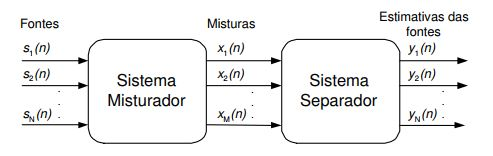
\includegraphics[scale=1.0]{fig221.JPG}\hspace*{\fill}
        \caption{Estrutura do problema de Separação Cega de Fontes.}
        \label{fig:structure}
    \end{figure}


\section{Aplicabilidade}
    Devido à generalidade do problema de BSS, várias aplicações podem ser atribuídas. Veremos, nesta seção, algumas aplicações de destaque das técnicas de BSS nas diferentes áreas.
    
\subsection{Biomedicina}
    Na biomedicina, a busca por métodos não-invasivos que ainda se mostrem confiáveis é um desafio. o EEG (Eletroencefalograma) e o ECG (Eletrocardiograma) são dois exemplos bem comuns de técnicas que satisfazem esta necessidade. Entretanto, é relativamente difícil captar apenas os sinais desejados quando os sensores são posicionados em uma determinada região do corpo humano, principalmente devido à interferência proveniente de sinais gerados por outras atividades fisiológicas.
       
    Uma forma de resolver este problema está na repetição da realização do exame, o que pode não ser viável em certas ocasiões, além de causar fadiga nos pacientes. O emprego de técnicas de BSS oferece uma alternativa eficiente, uma vez que o processamento é dado após a coleta dos dados e requer apenas um experimento.
    
    Existe uma expressiva gama de trabalhos acerca de separação de sinais biomédicos, o que evidencia sua importância.
    
\subsection{Telecomunicações}

    A BSS está diretamente ligada com um tema relevante em telecomunicações: a equalização de canais A idéia essencial de um sistema de comunicação é fazer com que a informaçãõ enviada por um transmissor possa ser obtida de maneira tão fiel ao original quanto possível por um receptor. Assim sendo, mitigar distorções introduzidas pelo canal é fundamental. Em outra estratégia, a equalização do canal, utiliza-se um filtro (equalizador) no receptor demodo que este seja capaz de anular os efeitos do canal. Em essência, o desenvolvimento de técnicas de equalização está intimamente relacionado à concepção de critérios que guiem o ajuste dos parâmetros livres do equalizador de modo que se obtenha uma boa estimativa do sinal transmitido.
    Por exemplo, em um dos paradigmas mais conhecidos, adota-se como critério a minimização do erro quadrático médio     entre a saída do equalizador e o sinal desejado, no caso, o sinal transmitido (Haykin, 1996). Os critérios presentes na equalização não-supervisionada (ou cega) utilizam, além dos sinais recebidos, apenas algumas informações estatísticas dos sinais transmitidos. Uma vantagem desta estratégia em relação ao paradigma supervisionado é a possibilidade de realizar o ajuste dos parâmetros concomitantemente com a transmissão dos dados
    
\subsection{Separação de sinais de áudio}

    Imagine a seguinte situação: uma pessoa se encontra em uma sala onde existem diversos grupos de pessoas conversando concomitantemente, como, por exemplo, em uma reunião. Além disso, há ruído de fundo gerado, por exemplo, por música ambiente e ecos no recinto. Apesar de todas essas interferências, o ser humano é capaz de distinguir a voz ou o som de interesse em um determinado momento. Essa habilidade é conhecida na literatura como \textit{cocktail-party effect} (B. Arons, 1992), justamente pela analogia com o cenário descrito.

    Este caso levou ao questionamento: será possível a um sistema de processamento artificial alimentado apenas por gravações de microfones posicionados pela sala distinguir o sinal de voz de uma pessoa qualquer? Ao passo que o cérebro humano resolve com certa facilidade este problema, o desenvolvimento de sistemas automáticos para realizar tal tarefa ainda corresponde a um complexo desafio.

\section{Modelagem Matemática do Problema}
    Neste capítulo, iremos descrever como o problema de BSS pode ser resolvido. Primeiramente, é necessário buscar modelos matemáticos capazes de expressar o comportamento do sistema em função do misturador e do separador.
    
    Considere que cada elemento do vetor $\mathbf{s}$($\mathpzc{n}$) = [$\mathbf{s_1}$($\mathpzc{n}$) $\mathbf{s_2}$($\mathpzc{n}$) \dots  $\mathbf{s_N}$($\mathpzc{n}$)] corresponde a um sinal da fonte emissora. Analogamente, representamos os sinais misturados pelo vetor  $\mathbf{x}$($\mathpzc{n}$) = [$\mathbf{x_1}$($\mathpzc{n}$) $\mathbf{x_2}$($\mathpzc{n}$) \dots  $\mathbf{x_M}$($\mathpzc{n}$)]. De forma generalizada, o sistema misturador pode ser representado pela expressão:

    \begin{equation}\label{eq:mixer}
        \mathbf{x}(\mathpzc{n}) = \mathcal{F}(\mathbf{s}(\mathpzc{n}), \mathbf{s}(\mathpzc{n-1}), \dots, \mathbf{s}(\mathpzc{n - L}), \mathbf{n}(\mathpzc{n}))
    \end{equation}
    
    onde o operador $\mathcal{F}$($\cdot$) descreve a ação do sistema misturador, L corresponde ao número de amostras passadas (memória) do vetor de fontes e o vetor $\mathbf{n}$($\mathpzc{n}$) corresponde ao ruído associado às fontes ou sensores do sistema.
    
    Vale ressaltar que a representação (\ref{eq:mixer}) tem caráter puramente didático, uma vez que não existem técnicas de BSS que lidem com todos estes efeitos representados e uma só vez. Em geral, as técnicas são aplicadas a casos específicos, isto é, versões simplificadas da formulaçao citada. Desta forma, torna-se necessário introduzir os conceitos de classificação de um sistema misturador para auxiliar na adequação do problema para o caso proposto por este trabalho.
    
    \textbf{Sistemas Lineares vs. Não-Lineares} O sistema misturador é dito linear se o operador  $\mathcal{F}$($\cdot$) respeita o princípio da superposição, conforme descrito abaixo:

        % Linearidade
        \begin{equation}\label{eq:linearity}
            \mathcal{F}(\mathbf{a_1}\mathbf{s_1}(\mathpzc{n}) + \mathbf{a_2}\mathbf{s_2}(\mathpzc{n})) = \mathpzc{a_1}\mathcal{F}(\mathbf{s_1}(\mathpzc{n})) + \mathpzc{a_2}\mathcal{F}(\mathbf{s_2}(\mathpzc{n}))
        \end{equation}

    para quaisquer constantes $\mathpzc{a_1}$ e $\mathpzc{a_2}$ e vetores $\mathbf{s_1}$ e $\mathbf{s_2}$. Caso contrário, o sistema é classificado como não-linear. 
    
     \textbf{Sistemas Instântaneos e Convolutivos} Nos casos em que o sistema depende de amostras passadas, isto é, L$>$0, o sistema é dito convolutivo. No caso em que L=0, o sistema é dito instantâneo.
    
     \textbf{Sistema Sub-Determinado, Determinado e Sobre-Determinado} Quando o número de sensores é maior que o número de fontes (M$>$N), tem-se o caso sobre-determinado. Analogamente, o caso sub-determinado corresponde ao caso em que (M$<$N). O caso em que (M=N) é considerado determinado.
     
     Apesar da característica principal da BSS ser a falta de informação sobre o processo de mistura, é fundamental ao menos um certo conhecimento sobre a estrutura do sistema misturador. Assim, é possível definir um separador estruturalmente capaz de reverter a ação do processo de mistura. Geralmente, este tipo de aplicação é obtido com base na aplicação de interesse. No caso deste trabalho, o problema de separação de sinais de áudio, o processo de mistura é notadamente convolutivo devido à reverberações do ambiente.
     
     A maioria dos trabalhos acerca da BSS abordam cenários com sistemas misturadores lineares e com o mesmo número de fontes e sensores, diferenciando-se basicamente no contexto de misturas instantâneas ou convolutivas. Apesar desta última classificaçãço desempenhar um papel fundamental na abordagem do problema, o  processo de mistura pode ser igualmente descrito matematicamente da seguinte forma:
     
     % Notação Matricial
     \begin{equation}\label{eq:xn}
        \mathbf{x} = \mathbf{A}\mathbf{s}
    \end{equation}
    
    onde a matriz $\mathbf{A}$ de dimensão $\mathpzc{N x N}$ é chamada de matriz de mistura. A diferença é que, no caso linear, os elementos da matriz $\mathbf{A}$ são constantes que multiplicam com as componentes do vetor de fontes $\mathbf{s}$ para formar as misturas $\mathbf{x}$, enquanto no caso convolutivo, os elementos da matriz $\mathbf{A}$ são filtros \textit{FIR} que representam o percurso realizado pela fonte até o sensor, devido à reverberação. Assim, tem-se uma convolução de cada um desses filtros com cada elemento do vetor de fontes $\mathbf{s}$. A despeito de sua simplicidade, esta classe de modelos é válida em uma vasta quantidade de problemas de BSS (\cite{ICA}). Além disso, é possível recuperar as fontes através da Análise de Componentes Independentes, que será visto na próxima seção.

\section{Análise de Componentes Independentes}
    Nesta seção serão apresentados os aspectos básicos da ICA, relacionando-a com alguns métodos semelhantes. Embora a ICA seja definida para o caso linear e convolutivo, trataremos apenas do caso linear, pois é o que condiz com a abordagem que queremos realizar, a de separação das fontes no domínio da frequência. Recomendamos ao leitor interessado em um estudo aprofundado sobre os aspectos teóricos da ICA a leitura do trabalho de Comon (Comon, 1994), responsável pela formalização matemática desse assunto, e as referências (\cite{ICA}, \cite{ICA3}).
    
    Os algoritmos ICA podem ser derivados através da estimativa da máxima verossimilhança \cite{ICAML} e da maximização da não-gaussianidade \cite{ICAgauss}. Apesar da maioria dos algoritmos serem desenvolvidos para trabalhar com números reais, podemos estende-los para lidar com números complexos. Para isto, é preciso escolher aprorpriadamente uma função \textit{G}.

\subsection{Definição}
    Devido à sua natureza recente, não é difícil encontrar ao menos duas definições distintas para a ICA na literatura. Entretanto, utilizaremos a definição que mais se aproxima com a aplicação que é o objetivo deste trabalho.
    
    \bigskip
    
    \textbf{Definição 2.5.1 (ICA)} A ICA de um vetor aleatório $\mathbf{x}$ = [$\mathbf{x_1}$ $\mathbf{x_2}$ $\dots$  $\mathbf{x_M}]^T$ consiste em determinar o segundo modelo generativo linear (ou modelo ICA):
    
    \begin{equation}\label{eq:simplifiedmixer}
        % Notação Matricial
        \mathbf{x} = \mathbf{A}\mathbf{s}
    \end{equation}
    
    onde os elementos de $\mathbf{s}$ = [$\mathbf{s_1}$ $\mathbf{s_2}$ \dots  $\mathbf{s_N}$]$^T$ são estatisticamente independentes entre si e $\mathbf{A}$ corresponde a uma matriz constante de dimensão M x N.

    \bigskip 
    
    Sob a hipótese de que os sinais fontes são estatisticamente independentes entre si, fica claro que os elementos de $\mathbf{x}$ não são mais independentes, devido ao processo de mistura. O ponto fundamental da aplicação da ICA diz respeito exatamente a esta constatação, no sentido de que essa metodologia se propõe a separar as fontes a partir da recuperação da independência. O sistema separador, a matriz $\mathbf{W}$, é ajustado de modo que as compomentes do vetor $\mathbf{y}$ de estimativas das fontes sejam as mais independentes possíveis entre si.
    
    Entretanto, esta abordagem levanta a seguinte questão: tornar as estimativas das fontes independentes implica necessariamente na recuperação das fontes? Foi Pierre Comon (Comon, 1994) que não só respondeu a esta pergunta, mas também forneceu todo o respaldo matemático necessário para o desenvolvimento da ICA e, por consequência, da BSS.
    A partir do teorema de Darmois, ele mostrou que é possível separar as fontes com base na recuperação da independência estatística, respeitando algumas condições para as fontes e para o sistema separador.

\subsection{Separabilidade}\label{sec:separability}

    O modelo descrito em \ref{eq:simplifiedmixer} é dito separado se, para toda matriz separadora $\mathbx{W}$ que resulte em um vetor $\mathbf{y}$ que tem os elementos estatísticamente independentes entre sim, tem-se que $\mathbf{y}$ = $\mathbf{Wx}$ = $\mathbf{\Lambda P s}$, onde $\mathbf{\Lambda}$ e $\mathbf{P}$ representam matrizes diagonal e de permutação, respectivamente. Assim, em um modelo separável, é possível obter as fontes através da ICA. Entretanto, é importante ressaltar que surgem duas ambigüidades associadas a este modelo: não é possível recuperar a ordem das fontes nem seus ganhos de escala. Mediante este problema, Comon \nocite{Common} (Comon, 1994) formulou o seguinte teorema, evidenciando as condições necessárias para que um sistema misturador linear seja separável:
    
    \bigskip
    
    \textbf{Teorema 2.5.1 (Separabilidade)} O modelo $\mathbf{x} = \mathbf{As}$ é separável se e somente se a matriz $\mathbf{A}$ possuir posto completo e, no máximo, um dos elementos do vetor $\mathbf{s}$ for gaussiano.
    
    \bigskip
    
    Este teorema inclui mais uma restrição à aplicação da ICA, que é a incapacidade de recuperar fontes gaussianas. Na próxima seção, trataremos da utilização de estatísticas de segunda ordem para realizar a separação e este problema será melhor ilustrado. Também discutiremos como a utilização da correlação, uma medida mais "fraca", não é capaz de resolver o problema, mas pode ser bastante útil numa etapa de pré-processamento.
  
\subsection{Técnicas baseadas em estatístiscas de segunda ordem aplicadas à BSS}

    Até a década de 1980, a maioria das técnicas de filtragem estatística eram baseadas em estatísticas de segunda ordem. Isto era devido à simplicadade matemática relacionada a este tipo de abordagem e ao fato de que modelos gaussianos de sinais eram praticamente os únicos utilizados. 
    
    Foi durante o desenvolvimento da teoria de filtragem não-supervisionada, dentro do contexto de identificação e equalização cega, que se chegou a conclusão de que, para resolver essa classe de problemas, era necessário utilizar de estatísticas de ordem superior (\textit{HOS}) \cite{HOS}. Em BSS, esse conhecimento é fundamental.
    
    Na seção anterior mostramos que o problema da BSS pode ser resolvido com base na independência estatística, isto é, através de \textit{HOS}, uma vez que a independência requer conhecimento da densidade de probabilidade e, por consequência, todas as estatísticas de uma variável aleatória. Entretanto, esta seção será voltada para a apresentação da abordagem utilizando apenas estatísticas de segunda ordem para BSS, mostrando que isto não é suficiente para a resolução do problema.
    
    \subsubsection{Descorrelação}
    Com base no modelo ICA apresentado em \ref{eq:simplifiedmixer}, obtemos a matriz de correlação entre as misturas, denotado por:
    
    \begin{equation}
        \label{eq:correlationmatrixforx}
        \begin{split}
        \mathbf{R_x} & = \mathpzc{E}\{\mathbf{xx^T}\}\\
                     & = \mathpzc{E}\{\mathbf{(As)(As)^T}\}\\
                     & = \mathpzc{E}\{\mathbf{Ass^TA^T}\} \\
                     & = \mathbf{A}\mathpzc{E}\{\mathbf{ss^T}\}\mathbf{A^T} \\
                     & = \mathbf{A}\mathbf{R_s}\mathbf{A^T} \\
                     & = \mathbf{A}\mathbf{A^T} \\
        \end{split}
    \end{equation}
    
    onde $\mathbf{R_s}$ corresponde à matriz de correlação do vetor das fontes. Como estamos sob a hipótese de que as fontes são estatísticamente independentes e de que as fontes possuem variância unitária, esta matriz é igual à identidade.
    
    Após passar por um sistema separador, a correlação entre as estimativas das fontes é descrita por:
    
        \begin{equation}
        \label{eq:correlationmatrixfory}
        \begin{split}
        \mathbf{R_y} & = \mathpzc{E}\{\mathbf{yy^T}\}\\
                     & = \mathpzc{E}\{\mathbf{(Wx)(Wx)^T}\}\\
                     & = \mathpzc{E}\{\mathbf{Wxx^TW^T}\} \\
                     & = \mathbf{W}\mathpzc{E}\{\mathbf{xx^T}\}\mathbf{W^T} \\
                     & = \mathbf{W}\mathbf{R_x}\mathbf{W^T} \\
        \end{split}
    \end{equation}
    
    Assim, para descorrelacionarmos as saídas do sistema separador, precisamos determinar $\mathbf{W}$ tal que $\mathbf{R_y = I}$. Solucionando a equação, chegamos à conclusão de que:
    
    \begin{equation}
        \label{separationmatrixsolution}
        \mathbf{W} = \mathbf{D}^{-\frac{1}{2}}\mathbf{E^T}
    \end{equation}
    
    Entretanto, se consideramos o caso em que o sistema separador é dado pela expressão $\mathbf{QW}$, onde $\mathbf{Q}$ corresponde a uma matriz ortogonal (i.e, sua inversa coincide com sua transposta). Substituindo na solução da equação \ref{correlationmatrixfory}, fica claro ver que o resultado permanece o mesmo. Isto mostra que a recuperação das fontes utilizando apenas a informação da descorrelação apresenta uma indeterminação relacionada com um fator ortogonal.
    
    A Figura \ref{fig:orthogonalproblem2} ilustra geometricamente o problema. Com este objetivo, exibimos as Figuras \ref{fig:orthogonalproblema}, \ref{fig:orthogonalproblemb} e \ref{fig:orthogonalproblemc} as distribuições conjuntas de duas fontes, as misturas e suas estimativas obtidas pelo processo de branqueamento, respectivamente. Como o sistema misturador linear é modelado por uma matriz, as misturas são geradas a partir de rotações e escalonamento das fontes. Apesar do braqueamento conseguir recuperar as escalas das fontes, ele não consegue recuperar a rotação devido à indeterminação referente a uma matriz ortogonal, cujo efeito é a rotação dos dados.
    
    Esta ineficácia na recuperação de fontes gaussianas mostra a limitação da estatística de segunda ordem. Entretanto, a aplicação do branqueamento como um pré-processamento pode ajudar bastante no processo de separação, visto que este faz aproximadamente metade do trabalho de separação.
    
  \begin{figure}
    \begin{subfigure}
    \begin{center}
        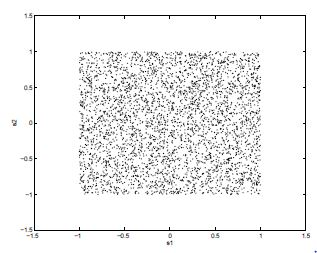
\includegraphics[scale=0.8]{distrib_fontes.JPG}
        \caption{Distribuição conjunta das fontes.}
         \label{fig:orthogonalproblema}
    \end{center}
     \end{subfigure}
     \begin{subfigure}
     \begin{center}
        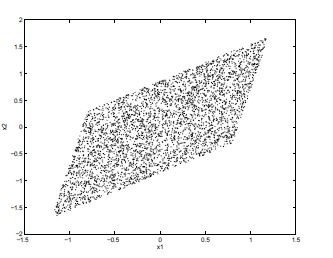
\includegraphics[scale=0.8]{distrib_misturas.JPG}
         \caption{Distribuição conjunta das misturas.}
        \label{fig:orthogonalproblemb}
    \end{center}
     \end{subfigure}
     \begin{subfigure}
     \begin{center}
        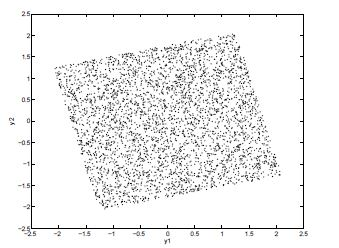
\includegraphics[scale=0.8]{distrib_estimat.JPG}
         \caption{Distribuição conjunta das estimativas obtidas a partir do braqueamento das misturas.}
                 \label{fig:orthogonalproblemc}
     \end{center}
     \end{subfigure}
     
  \caption{Tratamento da BSS considerando estatística de segunda ordem.}
  \label{fig:orthogonalproblem2}
\end{figure}

\subsection{Modelo de maximização da não-gaussianidade}
    
    Uma maneira de medir a independência entre duas estimativas de fontes é olhar sua não-gaussianidade, baseando-se no Teorema Central do Limite \cite{central}
    
    \medskip
    
    \textbf{Teorema 2.5.2 (Teormea Central do Limite)} Dadas \textit{n} variáveis aleatórias independentes $\mathpzc{x_i}$, formamos sua soma $\mathpzc{x = x_1 + \dots + x_n.}$. Esta é uma variável aleatória com média $\mathpzc{\eta = \eta_1 + \dots + \eta_n}$ e variância $\mathpzc{\sigma^2 = \sigma_1^2 + \dots + \sigma_n^2}$. O Teorema Central do Limite diz que, dentro de certas condições gerais, a distribuição $\mathbf{F(x)}$ de $\mathpzc{x}$  se aproxima de uma distribuição normal com a mesma média e variância à medida que \textit{n} cresce.
    
    \medskip
    
    Em termos práticos, quanto mais misturadas estiverem as fontes, mais gaussiana ela estará. Existem duas formas de medir a gaussianidade: a curtose e a negentropia. Por não ser o objetivo deste trabalho, apenas introduziremos o conceito de cada uma das abordagens e optaremos pela utilização da negentropia, devido à sua robustez em relação ao caso da curtose. Além disto, o algoritmo utilizado escolhido é o \textit{NaturalICA}, que é baseado na maximização da verossimilhança, que será visto na seção a seguir. Assim sendo, convidamos o leitor que esteja interessado no aprofundamento das abordagens, a leitura de \cite{LuizVictorio}.
    
    A curtose é uma estatística de quarta ordem que categoriza as distribuições como gaussiana, subgaussiana e super-gaussiana. Também pode ser interpretada como a inclinação da curva gaussiana. Entre os problemas referentes à abordagem da ICA na curtose, estão o problema do algoritmo baseado em um gradiente, fazendo com que o mesmo necessite uma sábia escolha de um passo de adaptação e podendo resultar em convergência lenta ou até mesmo divergência. Além disso, o problema com \textit{outliers}, que correspondem às observações da amostra que desviam completamente das demais, tem bastante influência na não utilização do método, uma vez que um \textit{outlier} pode mudar completamente a curtose.
    
    Já a abordagem da Negentropia é mais robusta, apesar de ser computacionalmente mais intensiva. Entretanto, existem aproximações simples que garantem um resultado satisfatório nesta abordagem. A entropia é um conceito da Teoria da Informação e está relacionada à incerteza associada à uma variável aleatória. Quanto maior o seu valor, mais aleatória é a variável. Um resultado fundamental da Teoria da Informação é de que uma variável contínua com distribuição gaussiana tem a maior entropia diferencial entre todas as variáveis de igual variância. Um problema da entropia diferencial é que seu valor é alterado quando a variável aleatória é multiplicada por uma constante. Para resolver este problema, introduzimos o conceito de negentropia, que é uma utilização da entropia de forma que fique invariante À qualquer transformação linear invertível. 
    
    Para esta abordagem, é comum escolher uma função não linear \textit{G} e incorpora-la à formulação tradicional do método de forma a simplificar o modelo e reduzir os custos computacionais.
    
\subsection{Modelo de estimação por máxima verossimilhança}

Os algoritmos que utilizam estimativa por ML não colocam nenhuma restrição na matriz separadora, assim podem chegar a resultados mais precisos. Baseiam-se na maximização da verossimilhança da matriz separadora $\mathbf{W}$.
